\section{LiveClips System Overview}
\label{sec:liveclips_system}

LiveClips takes as input a live streamed video and telemetry data for the software usage in the video. It extracts short clips showing bite-sized chunks of the artistic process, crops clips to thumbnail size, and ranks clips for recommendation based on their properties as well as the user's context. The current implementation of LiveClips extracts clips from a corpus of Making live streams, though we believe its approach can extend to other types of creative live streams as well. As our formative work showed, Making streams focus on the work being created, making them an appropriate candidate for exploring the potential of inspirational clips. In the current implementation, audio is removed to focus solely on the visual component of the videos, as our formative work showed that streamers often talk about irrelevant topics while working.

Our approach is tool-centric: each clip focuses on one tool and LiveClips recommends clips based on the user's tool use in the application. We focus on tools as a starting point, because prior work has demonstrated that short tool-focused clips can be effective for contextual learning~\cite{Grossman2010a} and creative software tasks are often centered around the use of different tools. The next section describes LiveClips' three user interface prototypes, and the following section describes the backend system.

\section{User Interfaces}
Based on the design space outlined in \autoref{sec:liveclips_designspace}, we present three alternative methods for displaying and recommending the video clips generated by LiveClips in creative software (\autoref{fig:liveclips_photoshop}).
All three methods provide a link to the original video source underneath each clip, so that users can easily access it if desired. Each interface was implemented as a prototype \textsc{html}/Javascript extension to Adobe Photoshop.

\begin{figure}[b!]
\centering
  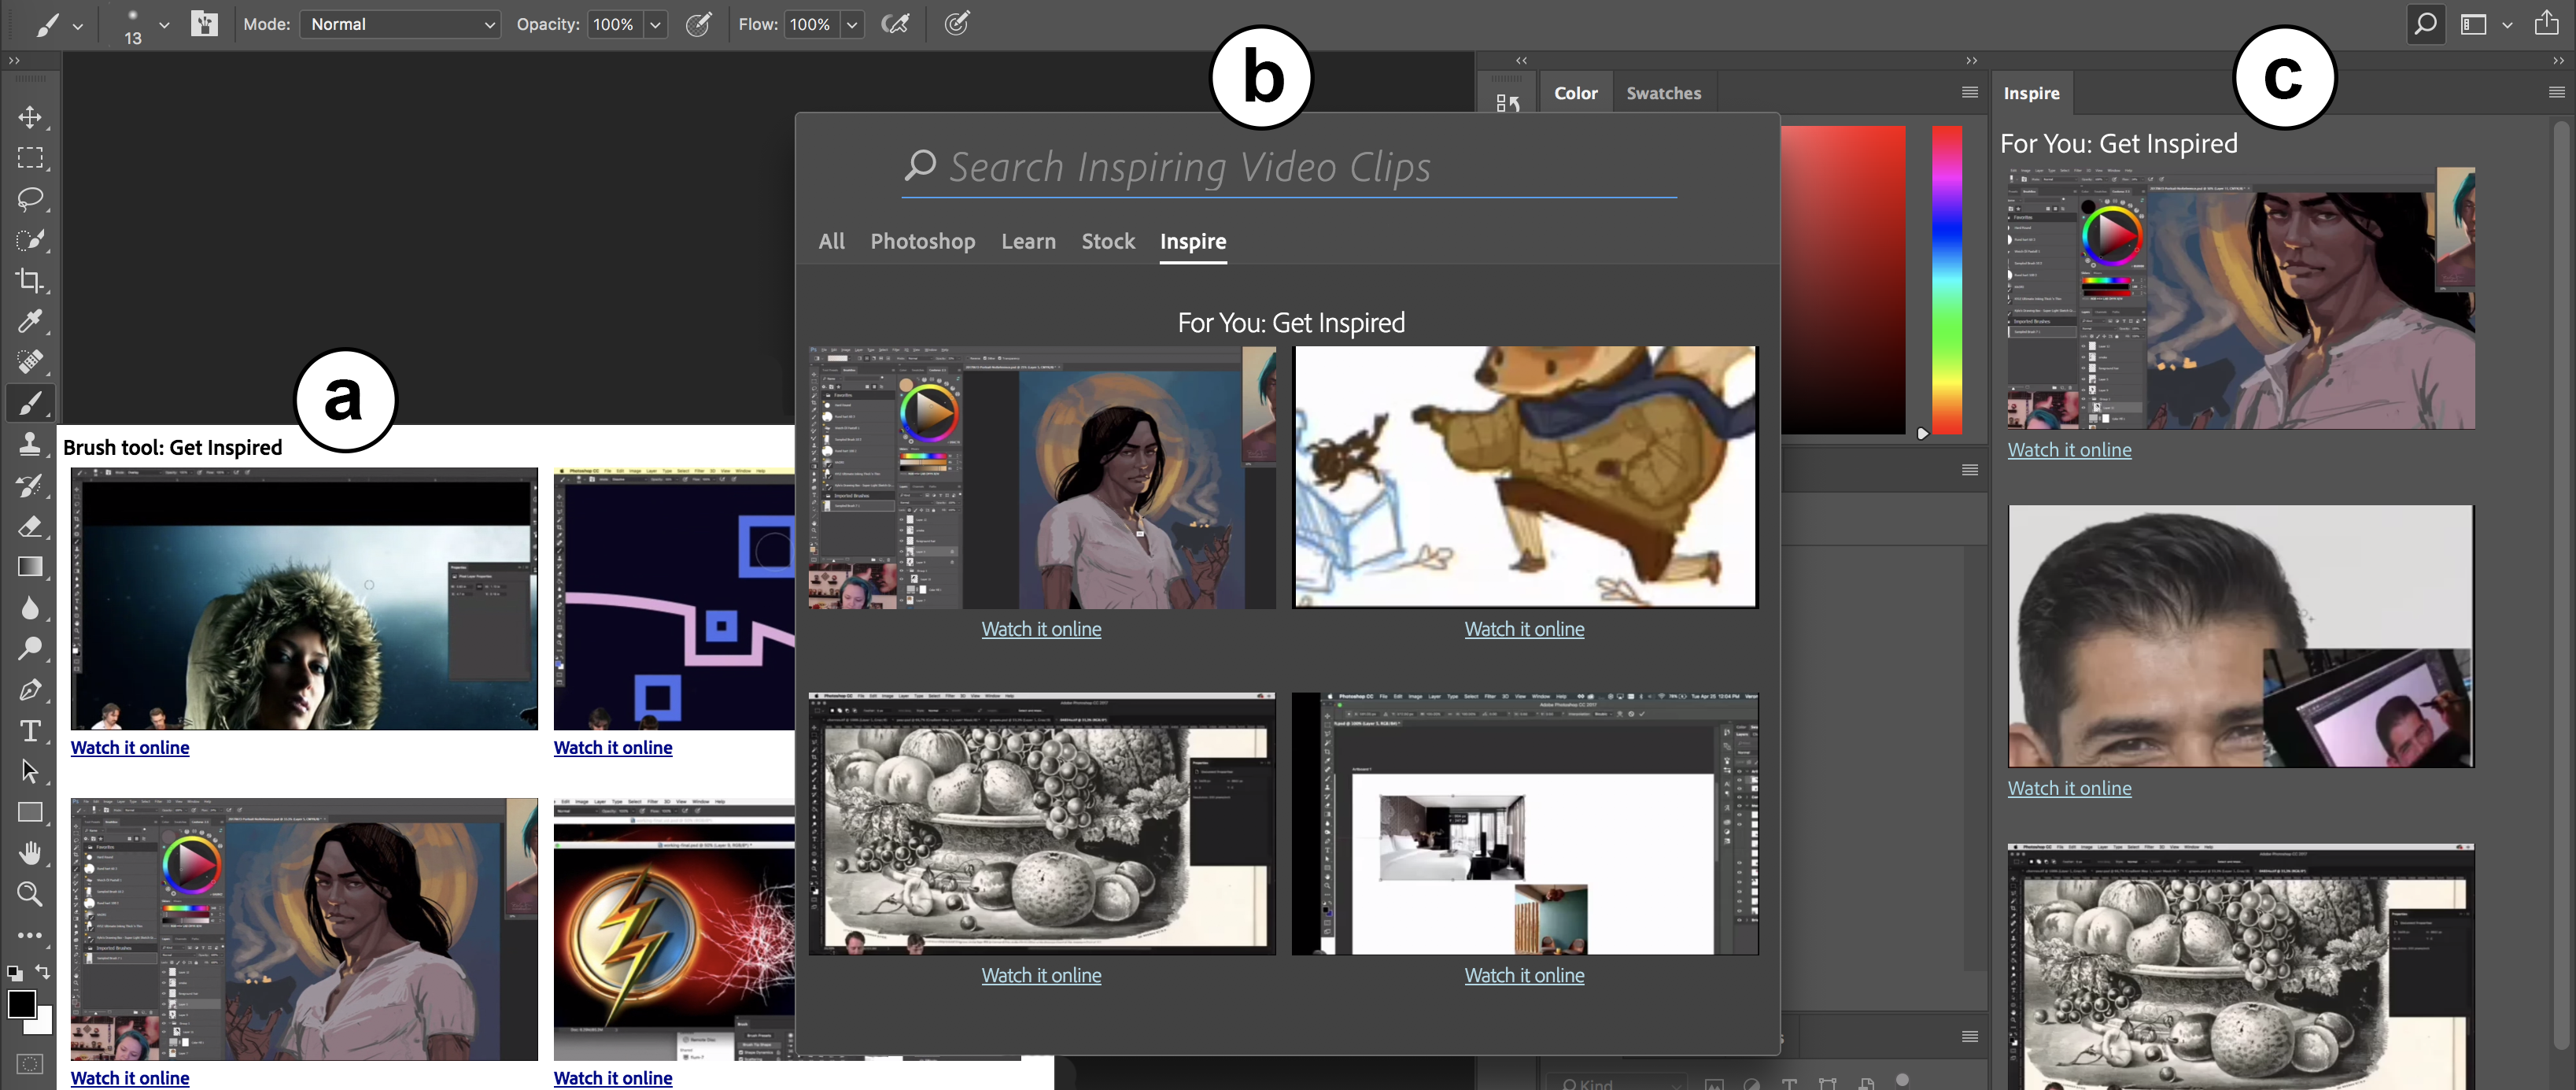
\includegraphics[width=\textwidth]{liveclips/figures/all_interfaces.png}
  \caption[LiveClips' three interface prototypes demonstrate how video clips taken from creative live streams can be embedded in software as inspirational examples, implemented here in Adobe Photoshop.]{LiveClips' three interface prototypes demonstrate how video clips taken from creative live streams can be embedded in software as inspirational examples, implemented here in Adobe Photoshop. a) Contextual tooltips: When hovering over a tool icon, clips of that tool being used are shown. b) On-demand search: Pressing Photoshop's search button or Ctrl-F brings up an extended search interface with task-level clip examples. c) Ambient side panel: an always-visible panel updates periodically with clip examples based on the user's recent tool use. }~\label{fig:liveclips_photoshop}
\end{figure}

\subsection{On-demand Search}
Many software applications provide in-application search, which allows users to search for application features, help, and/or recent documents. We augmented Photoshop's in-application search interface to present four clips when the search window is opened (\autoref{fig:liveclips_photoshop}b). Clips are selected based on the user's tool use during the entire work session. Users can also search the entire library of video clips from this window. This interface is the closest in concept to RePlay and ReMap's interfaces. As such, we expect this interface to be most useful in moments where the user is stuck and wants new ideas. Each video is displayed as a thumbnail showing the first frame and plays when clicked.

This interface has low visibility, and updates only in response to an explicit user action. It uses higher-level context to recommend examples. Playback requires intentional mouse clicks.

\subsection{Ambient Side Panel}
Since creative applications tend to include many panels, a natural location for examples is in a side panel (\autoref{fig:liveclips_photoshop}c). This interface explores examples that update ambiently as the user works. To avoid distracting the user during periods of focused work \cite{Chan2017}, the examples only update after the user has been idle for 10 seconds, indicating that they might be taking a break or trying to think of new ideas \cite{Siangliulue2015}. The panel shows four clips based on the user's recent tool use. Mousing over a clip plays it, providing a low threshold for interaction without distracting the user by playing video clips automatically.

This interface has high visibility, updates in response to implicit user actions, and uses mid-level context to recommend examples. Playback requires mouse movement without clicks.

\subsection{Contextual Tooltips}
For an interface that lies between an on-demand window and an always-visible panel, our third approach shows examples in tooltips that appear when the user hovers over a tool icon for 3 seconds (\autoref{fig:liveclips_photoshop}a). Inspired by ToolClips \cite{Grossman2010a}, we believe tooltips may be a useful location for video examples. They can be activated by the user with minimal effort, are easily dismissed, and will not display at all if the user is working quickly or activating tools with keyboard shortcuts.
Tooltips are a natural place for tool-centric examples; the video clips shown are based on the tool selected. Our implementation shows four clips when the user hovers over a tool, and clips play automatically when the tooltip appears.

This interface has mid-level visibility, updates on demand, uses low-level context (tools) to recommend examples, and requires no interaction for video playback. 

\section{LiveClips System for Generating Clips}
The LiveClips system comprises three stages: 1) extracting short 25-second clips based on tool use from long videos, 2) cropping clips so that they can be displayed at thumbnail size, and 3) ranking clips for the three interfaces described above (\autoref{fig:liveclips_system}). The main goal for these clips is to expose users to what is possible in their creative software, and inspire them with new ideas and ways to use the software's tools.

\begin{figure}[b!]
\centering
  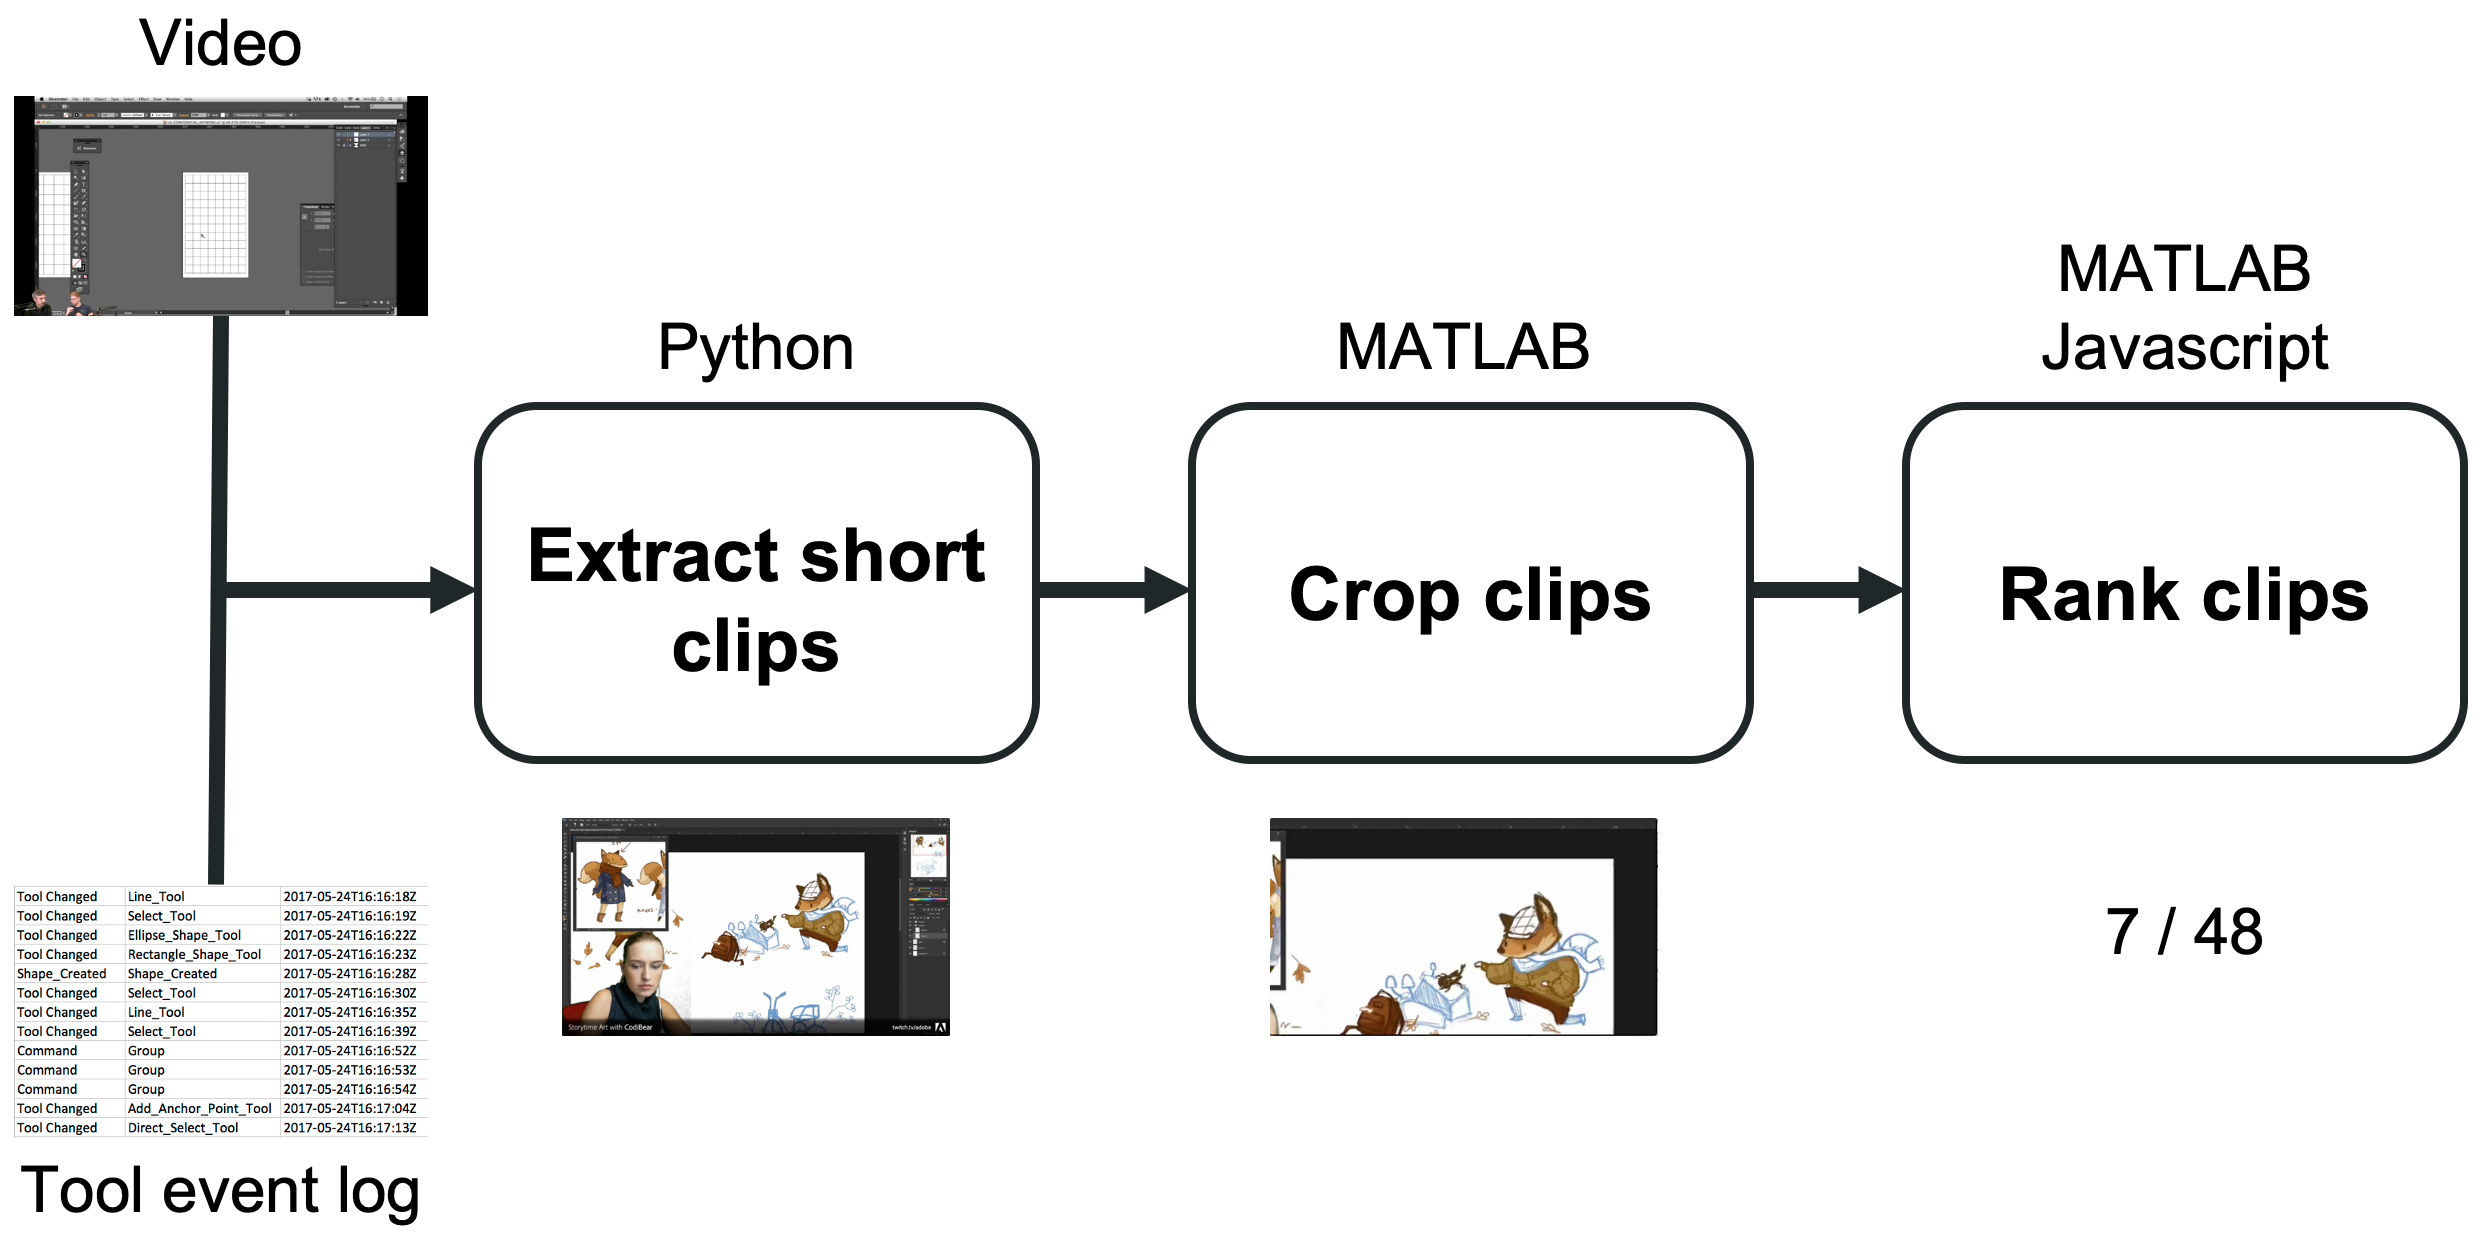
\includegraphics[width=0.9\textwidth]{liveclips/figures/liveclips_system.png}
  \caption[The LiveClips system takes as input a live streamed video and telemetry data for the tool usage in the video. It then: 1) extracts short clips based on tool use, 2) crops clips so that they can be displayed at thumbnail size, and 3) ranks clips for presentation.]{The LiveClips system takes as input a live streamed video and telemetry data for the tool usage in the video. It then: 1) extracts short 25-second clips based on tool use from long videos, 2) crops clips so that they can be displayed at thumbnail size, and 3) ranks clips based on their inspirational value and relation to the user's context. }~\label{fig:liveclips_system}
\end{figure}

Our approach uses a hybrid of telemetry (recorded usage data) and computer vision to understand and analyze the videos. We note that this could be accomplished entirely with telemetry (as in \cite{Grossman2010, Lafreniere2014}) by instrumenting the artists' software with detailed logging. Conversely, it could be accomplished entirely with computer vision, as prior work has shown that mouse movement and tool selection can be detected from videos alone \cite{Banovic2012, Pongnumkul2011}. In our case (which is not uncommon), we have some usage data that is not fully detailed. Our approach aims to be a catch-all that allows working with a mixed or inconsistent set of data. LiveClips removes all audio from clips during processing, focusing only on the visual component. This decision was motivated by our formative work finding that streamers talk about both relevant and irrelevant topics while working. While removing the audio risks removing potentially relevant narration, it avoids the challenges of properly segmenting narration that may or may not align with the work being shown.

\subsection{Available Data}
To develop and test LiveClips, we collected a sample dataset of creative live stream videos from the same two communities we analyzed in the formative work: the \textit{Creative} category on Twitch and \textit{Adobe Live} on YouTube. In an effort to make the sample as representative as possible, we collected videos from 17 different artists, and for two different software applications: Adobe Photoshop and Illustrator. Videos ranged in length from 30 minutes to 3 hours, giving us a total of 30 hours of video content from 17 different videos. 

All videos in our dataset were streamed either by Adobe (\textit{Adobe Live}) or by an artist supported by Adobe (\textit{Twitch Creative}). Therefore, for each video we had access to telemetry data produced by the artist's software at the level of tool usage, which includes time-stamped events for every selection and invocation of a tool (\autoref{fig:liveclips_usage}). Mouse clicks and canvas manipulation details were not available. Our dataset included the use of 36 different tools from the toolbars in Photoshop and Illustrator.  

\begin{figure}[b!]
\centering
  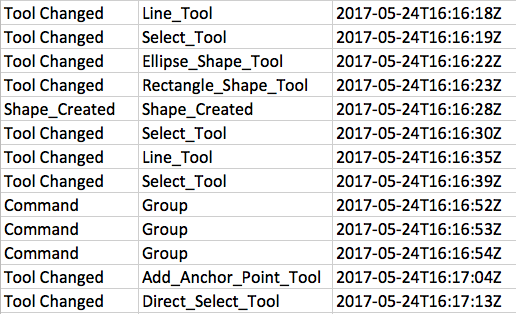
\includegraphics[width=0.5\columnwidth]{liveclips/figures/usage.png}
  \caption{A sample excerpt of the time-stamped usage data we had for each live stream video.}~\label{fig:liveclips_usage}
\end{figure}


\subsection{Extracting Clips}
To extract short clips, we use a heuristic approach based on work by Lafreniere \textit{et al.} \cite{Lafreniere2014}, who segment videos to create instructional clips of tool use. Our focus is on creating inspiring clips, which are different from instructional clips in that they require less attention to specific details (such as setting a tool's parameters) and more attention to the content being created. For the purposes of segmenting initial clips, our method is very similar to Lafreniere \textit{et al.}'s method. We focus on inspirational value in the cropping and ranking stages.

Given a tool, our goal is to create clips showing its use. First, we group all consecutive invocations of the tool and include the tool selection event if it happened within 10 seconds of the first invocation. We add 2 seconds of padding to the beginning so that the viewer can see the tool being selected or invoked. We then trim clips to 25 seconds, as prior work has indicated that 15-25 seconds is a desirable length for in-application video clip recommendations \cite{Lafreniere2014}. We also ignore the use of navigation tools (\textit{e.g.}, zoom, scroll, select) as these tend to happen frequently in visual software as part of other tasks. We shorten clips where the context likely changed before it was over, \textit{i.e.} if a document was closed or opened. If a clip is shorter than 15 seconds, we remove it.

This heuristic approach sometimes fails. For example, live streaming artists often work meticulously with one tool for long periods of time (\textit{e.g.}, a brush tool to create artwork), making incremental changes that over time create a more drastic and impressive change. The first 25 seconds of this may not be very inspiring, so we also explore an alternative method for creating clips that brings the focus away from the specifics of a tool's use, and toward the content being created: for instances where a tool is used consecutively for longer than 25 seconds, we extract the entire section where that tool is used, and speed it up to be 25 seconds long. We refer to these as timelapse clips.

In our sample set of 30 hours of video, the above two methods combined produced 1,727 clips, 484 of which were timelapses. This is comparable with Lafreniere \textit{et al.} \cite{Lafreniere2014}, who generated approximately 2500 clips from 25.5 hours of footage. LiveClips generated between 1 and 939 clips for each of the 36 tools in our telemetry dataset.

\subsection{Cropping Clips}
To present examples within an application, they have to be easily viewable by the user. A main design challenge with contextual clip recommendations is the space constraint: prior research has shown that in-application video clips should be unobtrusive and not take up too much of the user's screen \cite{Grossman2010a}. Since live streamed videos typically include the artist's entire screen, simply resizing them to a small thumbnail size will make most of the interesting detail hard to see. Existing methods for cropping videos to a good thumbnail size include cropping it to only the region of the document that changes in the clip \cite{Grossman2010} or cropping to only relevant UI regions \cite{Chi2012}. While more animated effects such as ``pan and zoom'' might be appealing for providing both context and detail, Chi \textit{et al.} \cite{Chi2012} found that too much animation is disorienting for brief video clips.

Since prior work has shown that visible change is an important factor affecting the usefulness of a video clip \cite{Lafreniere2014}, LiveClips attempts to crop each video clip to the area that changes most in the clip, so that the viewer's attention is drawn to the changes that are happening. For inspiration, we are mainly interested in visual change on the canvas. However, there are many other types of visual change that happen in these videos, such as switching windows, opening dialogs, and zooming in and out, and movement of the streamer in the webcam view of their face. Some of these changes (\textit{e.g.}, zooming) are simply uninteresting, and others (\textit{e.g.}, setting parameters in a dialog) may be helpful in a tutorial but are less interesting for short inspirational clips. 
 % Though users might want to see more specifics when they try and follow the artist's method, they will only reach this point if they find the content inspiring in the first place. In such situations, they can click go to the source video and watch the full original video on the Web. 
%
LiveClips therefore excludes these types of change before identifying the area that exhibits the most visual change. This leaves canvas changes and other UI changes. Although we are primarily interested in canvas changes, we leave the task of separating these from UI changes to future work.

To filter out these ``uninspiring'' visual changes, LiveClips uses computer vision to exclude visual change caused by navigational movement, changing application windows, and the artist moving in the webcam view. To detect navigation events, LiveClips does simple feature detection and point feature matching in \textsc{matlab} across consecutive frames to identify and exclude frames where there is a significant amount of motion (likely due to panning or zooming). To detect application window changes, LiveClips identifies moments where more than 90\% of the pixels change between two consecutive frames, and ends the clip before this change occurs. To detect change caused by the artist's webcam view, LiveClips uses face detection in \textsc{matlab} to locate faces that are consistently present in a bottom corner of the screen throughout the video, and mask out the corner containing those faces. The bottom corner is the customary place for streamers to place the webcam view of their face, and all the videos in our formative analysis as well as our implementation dataset either did not show the artist's face or showed it in a bottom corner, so this is a reasonable assumption for creative live streams.

To determine the area of most change after filtering out uninspiring changes, LiveClips first calculates the pixel-wise difference between each pair of consecutive frames in the video clip. It then computes the average difference over all of these difference frames. There are many changes around the edges of a clip where artists open menus and panels, but these are not very interesting. The interesting changes are on the canvas, which is typically in the middle of the screen. Thus, LiveClips trims off 100 pixels from all four sides. Next, LiveClips further trims off all sides where the pixel values in the average difference frame are less than a given threshold (which we set to 1/4 of the maximum value in the frame). This allows us to avoid specifying a desired crop size, since some clips may be already zoomed in on the part of the canvas being changed, requiring minimal cropping, whereas others may be zoomed out, requiring substantial cropping to highlight the changing area. \autoref{fig:liveclips_change} shows an example of the average difference frame from a clip and the crop that results from it.

\subsection{Ranking Clips for Recommendation}
The set of candidate clips generated is much too large to be useful, as only a few videos will eventually be shown to the user at any given time. As Lafreniere \textit{et al.} \cite{Lafreniere2014} found, over 50\% of automatically selected clips are of poor quality, so choosing good clips from the candidate set is an important step. This section outlines the criteria LiveClips uses to rank clips.

\subsubsection{Time in the original video}
Live streamed videos are several hours long and often show an entire project happening from start to finish. The closer an artist is to the end of their project, the more finished content they are likely to have on their canvas, and thus the more inspiring it is likely to be% (figure showing comparison if time)
. For each clip, LiveClips divides the start time of the clip by the total length of the video to obtain a number between 0 and 1 indicating how far along in the video the clip occurs. Larger numbers are better because they indicate that the clip occurs closer to the end.

\subsubsection{Amount of visual change}
 Lafreniere \textit{et al.} \cite{Lafreniere2014} found that showing clear visual change in short clips was most closely correlated to user preference. To determine how much visual change a given clip shows, LiveClips takes the cropped difference frame generated in the previous stage (\autoref{fig:liveclips_change}), and averages it across the $x$ and $y$ dimensions to obtain a numeric value representing the average amount of change in that clip (a larger number = more change).
 
\begin{figure}[b!]
\centering
  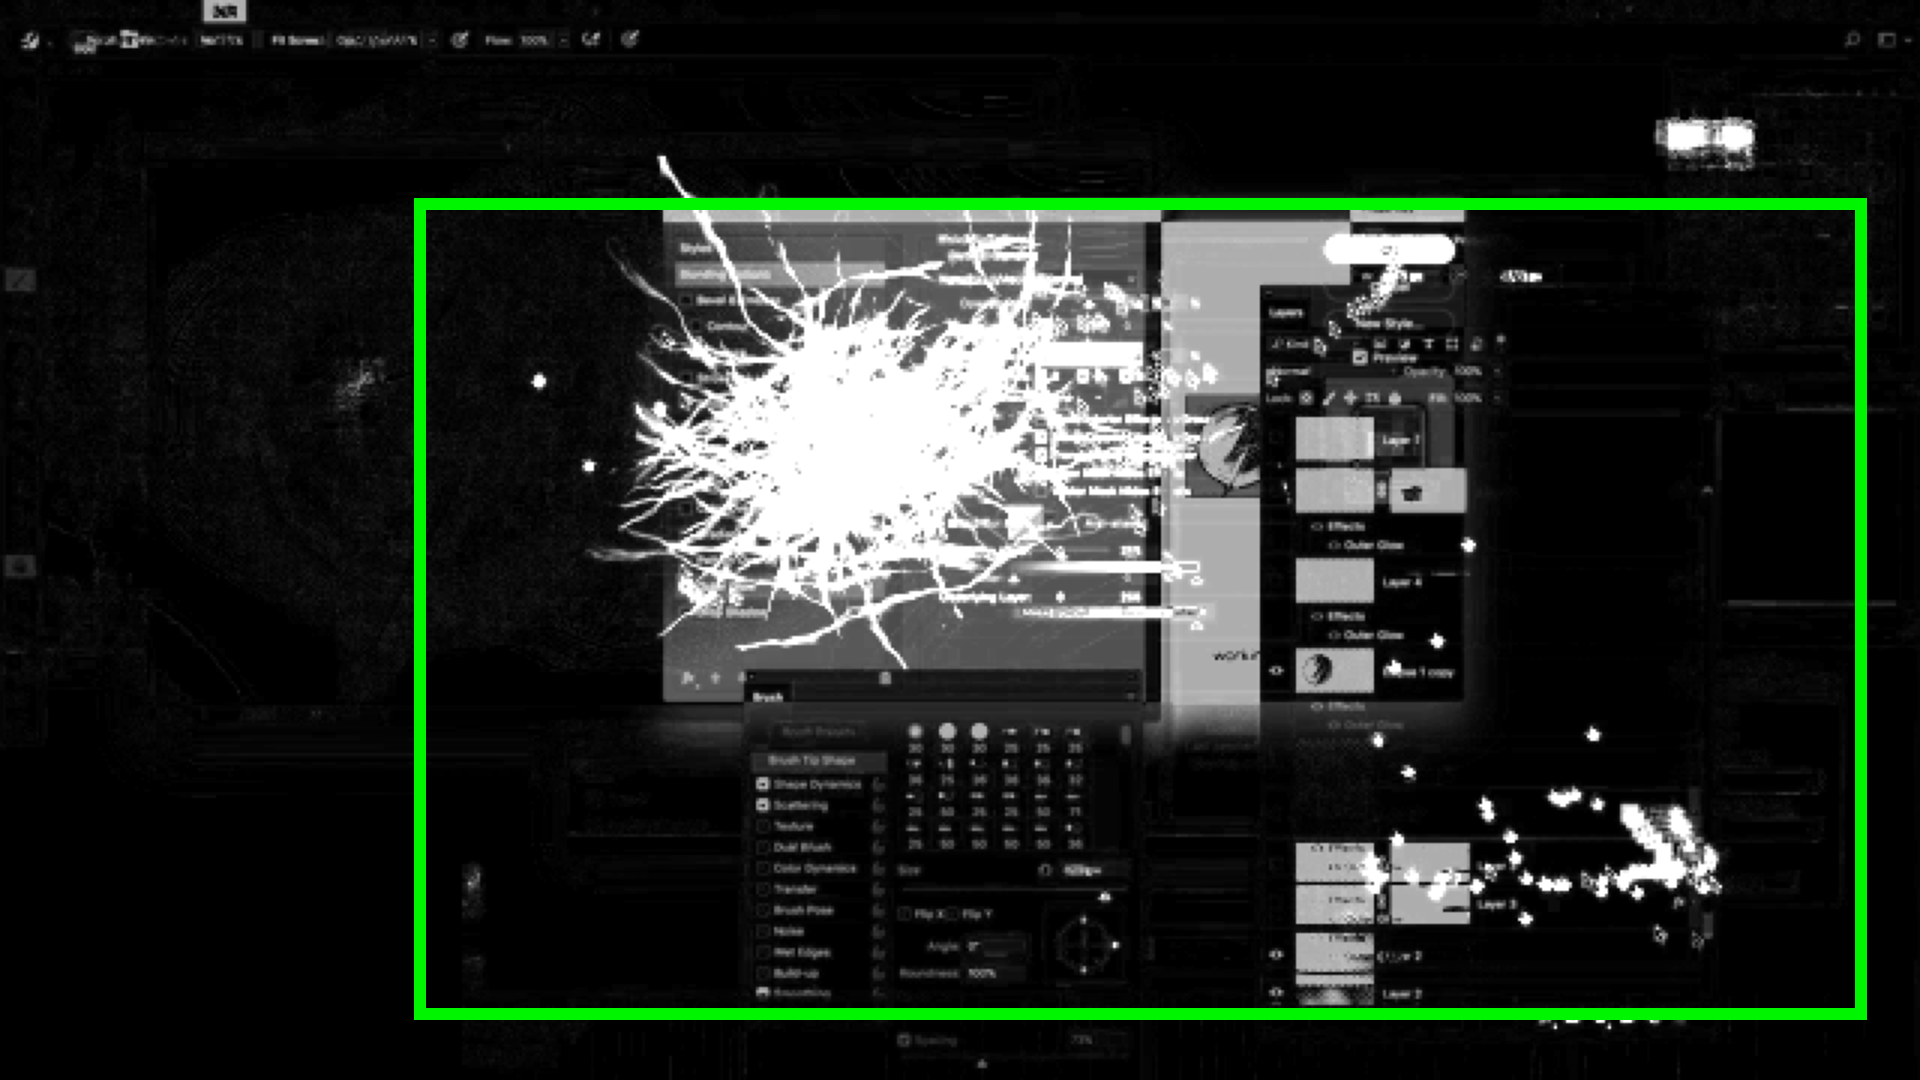
\includegraphics[width=0.7\columnwidth]{liveclips/figures/change.png}
  \caption[An example of a clip's visual change averaged across time (with change caused by navigation, application window switching, and the artist's face moving removed).]{An example of a clip's visual change averaged across time (with change caused by navigation, application window switching, and the artist's face moving removed). From the brightness values of the pixels, we can see that the artist opened some dialogs, and drew some lightning strokes. The green box shows how LiveClips crops the clip to focus on the area that is changing. }~\label{fig:liveclips_change}
\end{figure}

\subsubsection{User context}
User context is the final factor for selecting which video clips to present to the user. This metric varies in each of our three prototypes, to explore different levels of user context. LiveClips' current implementation uses tool use to measure context. LiveClips first calculates a ``total'' score for each clip by normalizing the time and visual change scores from above to be between 0 and 1, then taking the average. (For simplicity, we weight the two metrics evenly.) 

\textbf{Low-level context:} The contextual tooltips interface uses low-level context to recommend examples; video clips are selected based on the tool that the user hovers over. For a given tool, LiveClips orders all clips of that tool by total score, then picks the top four clips. LiveClips requires that all examples come from different source videos, to ensure a variety of content. If some of the top examples are from the same original video, the system goes down the list until it has a set from four different source videos. %In practice, this rarely happens. 

\textbf{Mid-level context:} The ambient side panel uses mid-level context to recommend examples; video clips are selected based on the last four tools the user has used. For each of those tools, LiveClips chooses the clip with the highest total score. If some of these clips are from the same original video, LiveClips instead picks the next top clips that are from different videos, to ensure variety.

\textbf{High-level context:} The on-demand search interface uses high-level context to recommend examples; the user's entire session of tool use is taken into account as well as the entire video from which each clip was extracted. %Many tools can be used for a variety of tasks; for example the brush tool in Photoshop could be used for making a digital painting, or for brushing on a mask to edit a photograph. It is likely that the overall distribution of tools used differs for the above two tasks: a user making a painting would likely spend most of their time using the brush tool and eraser tool, whereas a user editing a photograph might spend some time with the brush tool, and other time with tools such as the clone stamp and the spot removal tool. To recommend videos that more closely match the user's overall task, we therefore look at the time distribution of tool use in each video and compare it with the user's distribution of tool use. 
For each full-length video, we store the overall percent of time spent using each tool, and compare this with the overall percent of time the user has spent using each tool in their current session. To measure the ``difference'' between a video and the user's session, we sum the absolute differences between percentages for each matching tool (each is a number between 0 and 1), and for every tool used in the video that the user has not used at all, we add 1 to the sum. The video with the smallest difference sum therefore represents the closest match to the user's task. LiveClips chooses the live stream videos with the four smallest difference sums. From each video it picks the  clip with the highest total score.% that shows a tool that the user has used in the session.

%To make recommendations LiveClips recommendation engine compares all of the user's recent activity (\textit{e.g.}, which tools are used) to the overall activity in the live stream from which the the clip was extracted. 
%Inspired by CommunityCommands \cite{Li2011}, we consider only usage from the current session, which we define as the time since the user opened the application. For each video, we calculate the percent of time spent using each tool and compare this distribution with the percent of time the current user has spent using each tool. We select the top four videos whose distributions match most closely with the user's, and from each video we select the top ranked clip that shows a tool the user has used. 


%Second method: Recommendations are chosen based on the user's recent tool use, at a lower level than the search interface; every time the the recommendations update, it chooses the top ranked clip for each of the last four tools the user has used.